
%(BEGIN_QUESTION)
% Copyright 2010, Tony R. Kuphaldt, released under the Creative Commons Attribution License (v 1.0)
% This means you may do almost anything with this work of mine, so long as you give me proper credit

Suppose a 2.5 horsepower electric motor powered by 240 VAC (single-phase) power is used to turn a pump:

$$\includegraphics[width=15.5cm]{i04755x01.eps}$$

Using the conversion factor of 746 watts to one horsepower, calculate the amount of AC current drawn by the motor at full power (assuming perfect efficiency).  

\vskip 10pt

If the motor were only 90\% efficient (90\% of the applied power performing mechanical work, and 10\% of the applied power wasted in the form of heat), how much AC current would it draw at full power then?

\vskip 10pt

Program a computer spreadsheet (e.g. Microsoft Excel) to calculate the same ideal and real current values requested above.  Build the spreadsheet page so that all the given values in this problem (2.5 HP, 240 VAC, and 90\% motor efficiency) may be edited by the user, allowing the spreadsheet to be used to calculate ideal and real motor currents for a variety of different motor scenarios.

\vskip 20pt \vbox{\hrule \hbox{\strut \vrule{} {\bf Suggestions for Socratic discussion} \vrule} \hrule}

\begin{itemize}
\item{} Identify which fundamental principles of science, technology, and/or math apply to each step of your solution to this problem.  In other words, be prepared to explain the reason(s) ``why'' for every step of your solution, rather than merely describing those steps.
\item{} In any electrical device less than 100\% efficient, where does the ``lost'' energy go?
\item{} What design alterations might be made to an electric motor to increase its efficiency?
\item{} Describe the benefit of using computer spreadsheet programs such as Excel to perform calculations such as this, based on your experience using a spreadsheet to model this simple motor circuit.  How helpful do you think this might be on the job?
\end{itemize}

\underbar{file i04755}
%(END_QUESTION)





%(BEGIN_ANSWER)

A good way to convert horsepower into watts using the 746 conversion factor is to set up the equality in the form of a ``unity fraction'' to cancel units:

$$\includegraphics[width=15.5cm]{i04755x02.eps}$$

This cancellation technique ensures the multiplication and/or division is done properly, with the units showing you exactly how the fraction {\it must} be set up to properly cancel the undesired unit (horsepower) and replace it with the desired unit (watts).

\vskip 10pt

$I$ = 7.77 amps of current (assuming 100\% efficiency).

\vskip 10pt

$I$ = 8.63 amps of current (assuming 90\% efficiency).

\vskip 30pt

Here is a sample spreadsheet page, showing one possible layout for the values:

$$\includegraphics[width=15.5cm]{i04755x03.eps}$$

\begin{itemize}
\item{} {\bf Cell R1C5 formula:} {\tt = R1C2 * 746 / R2C2}
\item{} {\bf Cell R2C5 formula:} {\tt = R1C5 / R3C2}
\end{itemize}

Note that the use of ``R1C1'' spreadsheet row/column labeling is arbitrary; one may use the more customary ``A1'' letter/number labeling if desired.  There are some advantages to numbered row/column labels in more advanced spreadsheet programming, however, and so I recommend this style over the letter/number style.

%(END_ANSWER)





%(BEGIN_NOTES)


%INDEX% Electronics review: AC motor horsepower calculation

%(END_NOTES)

